\chapter{Laboratório 2}

\section{Sobre o problema}
O objetivo desse sistema é mensurar o nível de iluminação de um local utilizando o sensor LDR.
Quanto maior o nível de luz incidida, mais led's deverão ser acesos.

\section{Fundamentos teóricos}
\subsection{Sensor LDR}
O LDR (\textit{Light Dependent Resistor}) é um componente eletrônico passivo -- sem polaridade --, cuja resistência varia conforme a intensidade da luz que incide sobre ele.
A medida que a intensidade da luz incidida aumenta, a sua resistência diminui. \cite{https://pt.wikipedia.org/wiki/LDR}

\subsection{Conversor analógico-digital (ADC)}
Em resumo, o ADC é uma funcionalidade que converte uma tensão analógica em um determinado número. O Intel Galileo/Arduino possui 10 bits de precisão, portanto,
pode detectar ($2^{10}$ = 1024) níveis discretos analógicos. Isso significa que qualquer tensão (0 -- 5 V) que entre no pino ADC do Intel Galileo, será convertido em um
número de 0 a 1023. \cite{https://learn.sparkfun.com/tutorials/analog-to-digital-conversion}

\textbf{Fórmula:}

\begin{equation}
\frac{\textrm{Resolução do sistema}}{\textrm{Tensão do sistema}} = \frac{\textrm{Leitura ADC}}{\textrm{Tensão analógica medida}}
\end{equation}

Portanto, para o Intel Galileo, tem-se:

\begin{equation}
\frac{1023}{5} = \frac{\textrm{Leitura ADC}}{\textrm{Tensão analógica medida}}
\end{equation}


\section{Pré-requisitos}
\begin{itemize}
                \item Conversor digital-analógico;
                \item Operadores lógicos;
				\item Instrução condicional simples (se/então);
                \item Saída digital.
\end{itemize}
 
\section{Material necessário}

\begin{itemize}
	\item Intel Galileo;
	\item Protoboard;
	\item Jumpers ou fios;
	\item 1x resistor de 10 k$\mathrm{\Omega}$ e 4x resistores de 220 $\mathrm{\Omega}$;
	\item 4x led's (preferencialmente de cores diferentes);
	\item 1 sensor LDR.
\end{itemize}

\section{Circuito montado}

Os led's devem ser mantidos o mais longe possível do sensor LDR, evitando assim, que a luz emitida por eles interfira na medida feita pelo sensor.

\begin{figure}[!htb]
\centering
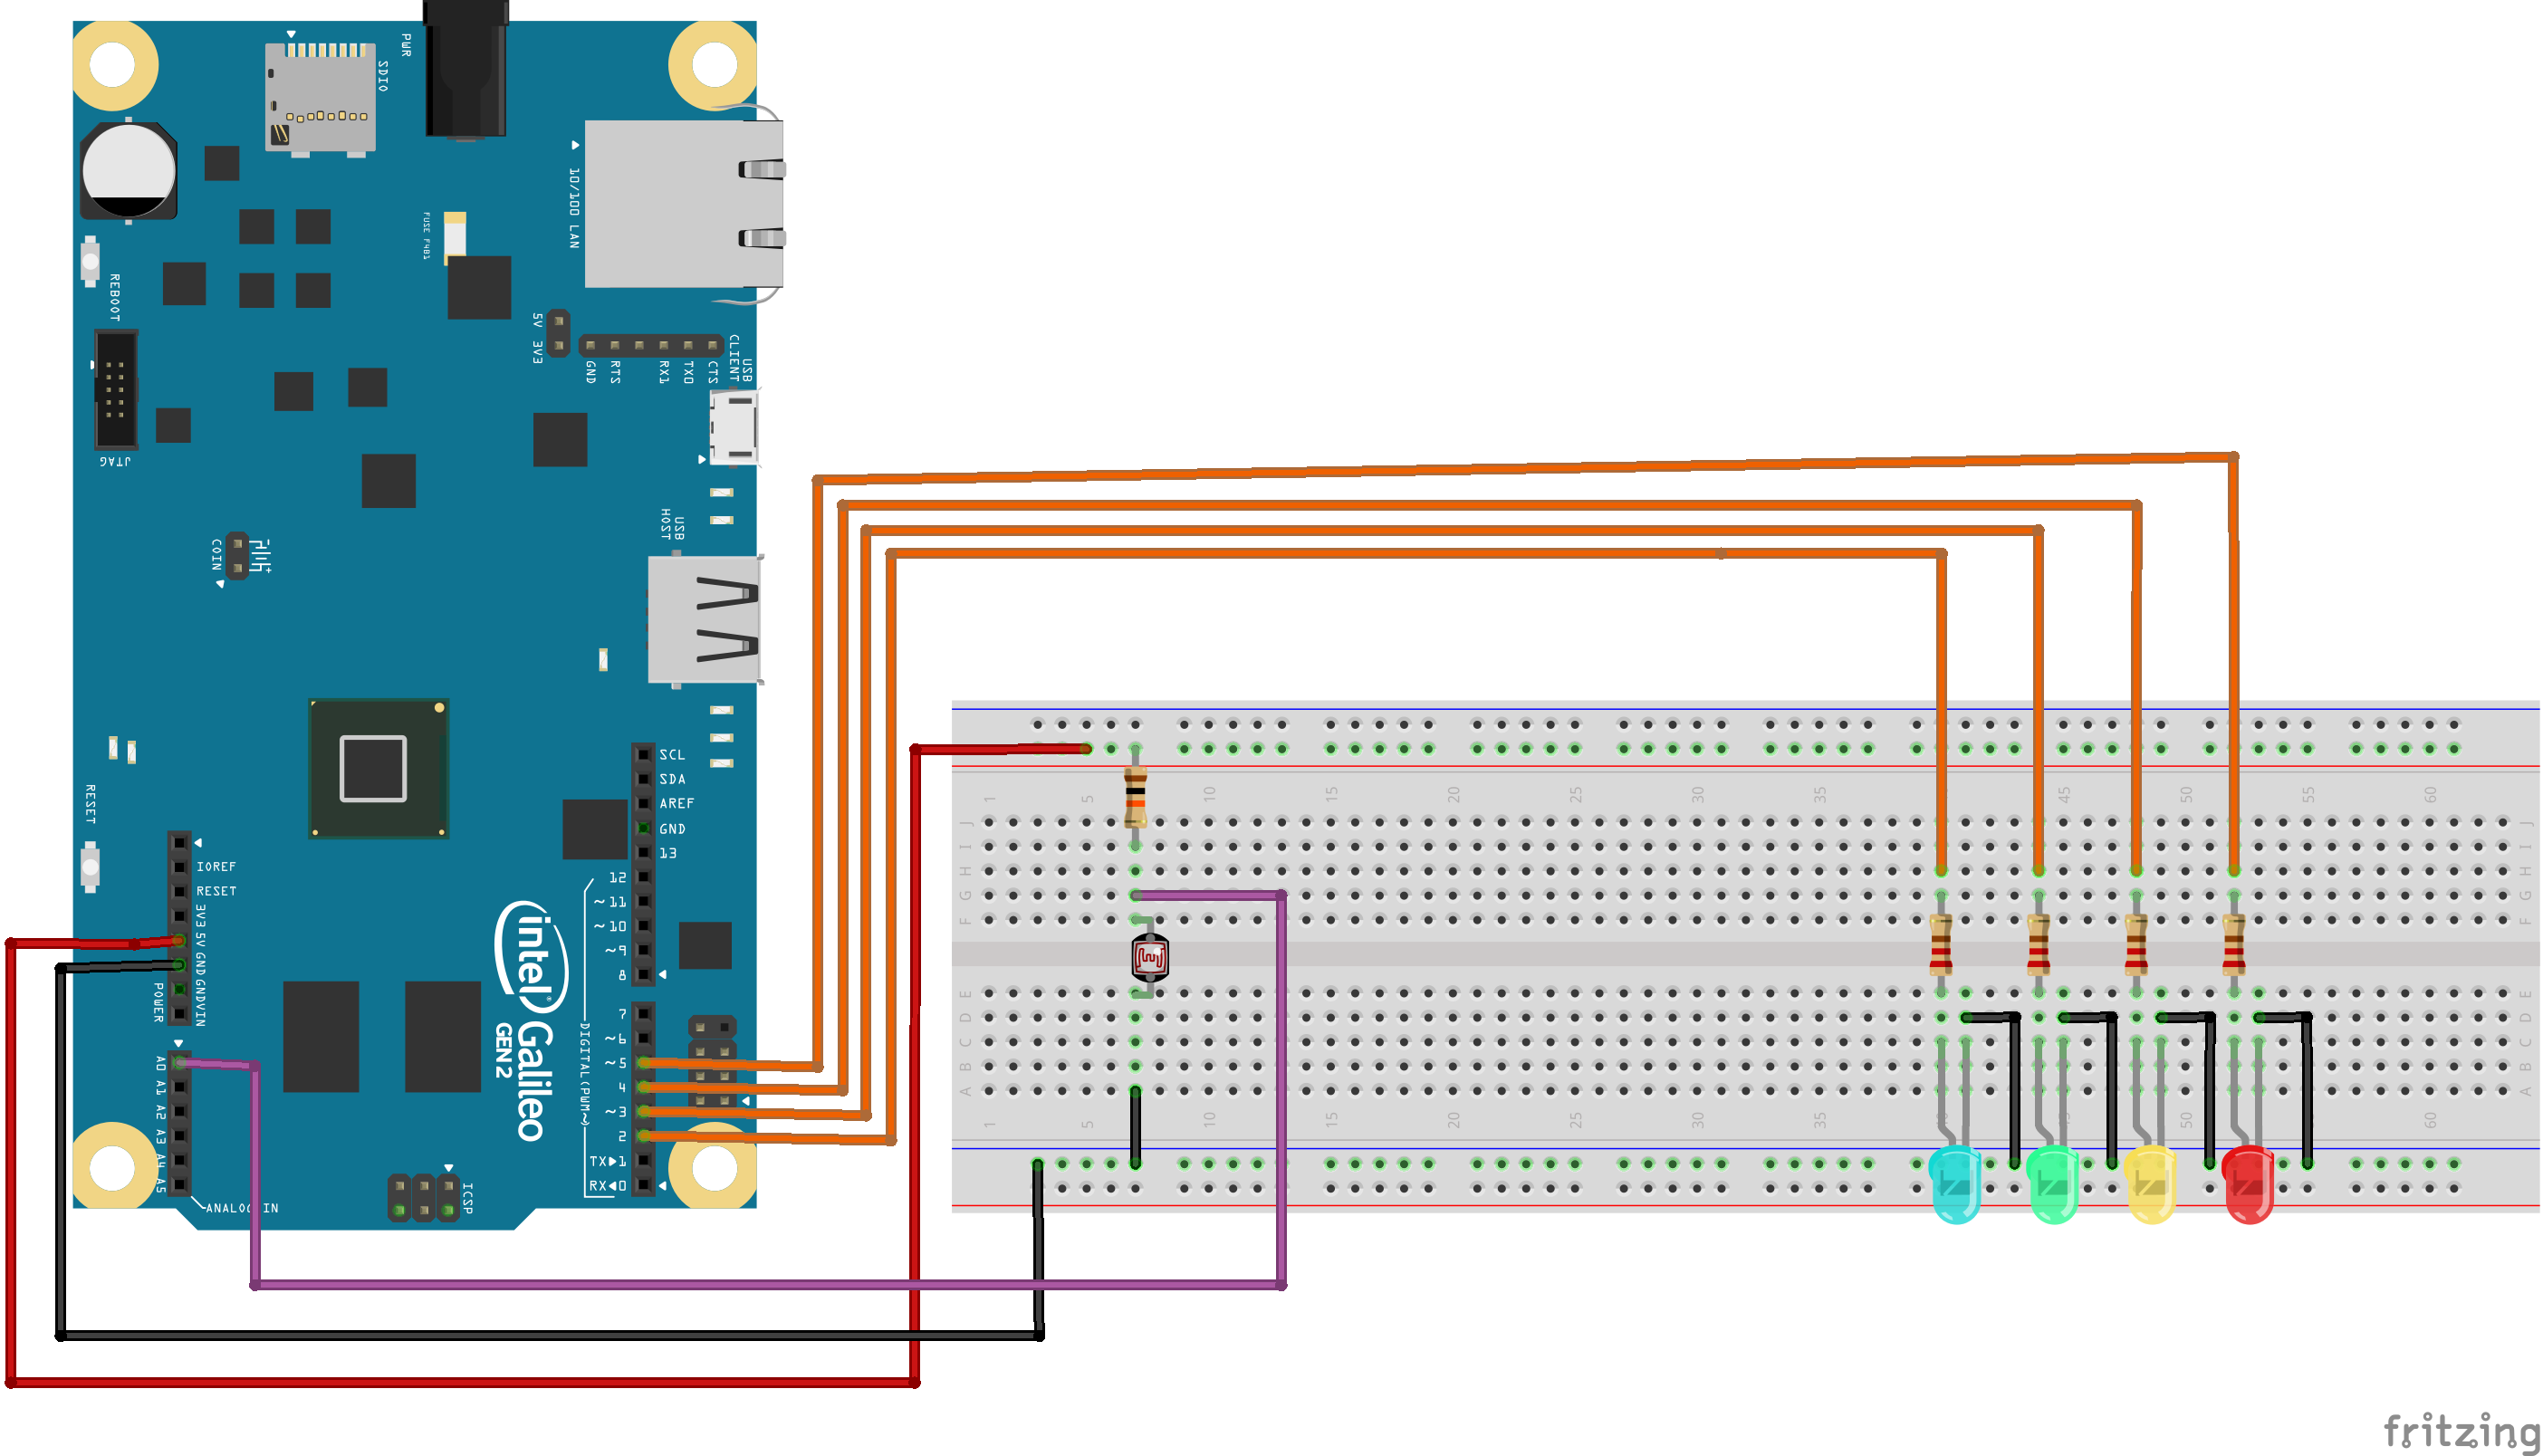
\includegraphics[scale = 0.6]{lab2_charles/nivel_iluminacao_bb.png}
\caption{Montagem do circuito utilizando o software Fritzing}
\label{circuito}
\end{figure}

\section{Código}

\lstset{inputencoding=utf8/latin1, breaklines = true}
\lstinputlisting[float=h]{lab2_charles/lab2_galileo.ino}

